%\documentclass[12pt,a4paper,addpoints]{exam}
\documentclass[12pt,a4paper,addpoints,answers]{exam}
\usepackage[T1]{fontenc}
\usepackage[utf8]{inputenc}
\usepackage[spanish]{babel}
\usepackage{multirow}
\usepackage{graphicx}
\usepackage{xcolor}
\usepackage{listings}
\usepackage{upquote}
\usepackage{xcolor}
\usepackage{listings}
\usepackage{amsmath}


% Definición de colores
\definecolor{keywordcolor}{rgb}{0.1,0.1,0.8} % Azul para palabras clave
\definecolor{stringcolor}{rgb}{0.8,0.1,0.1}  % Rojo para cadenas
\definecolor{commentcolor}{rgb}{0.1,0.6,0.1} % Verde para comentarios

% Configuración de listings
\lstdefinestyle{mysqlstyle}{
  basicstyle=\ttfamily\footnotesize,          % Estilo básico
  keywordstyle=\color{keywordcolor}\bfseries, % Estilo para palabras clave
  commentstyle=\color{commentcolor}\itshape,  % Estilo para comentarios
  stringstyle=\color{stringcolor},            % Estilo para cadenas
  showstringspaces=false,                     % No mostrar espacios en cadenas
  tabsize=2,                                  % Tamaño de tabulación
  breaklines=true,                            % Dividir líneas largas
  morestring=[b]",                            % Cadenas con comillas dobles
  literate={ñ}{{\~n}}1,                       % Permite el carácter "ñ"
  morekeywords={SELECT, INSERT, UPDATE, DELETE, FROM, WHERE, JOIN, INNER, LEFT, RIGHT, ON, GROUP, BY, ORDER, ASC, DESC, CREATE, TABLE, DROP, ALTER, DATABASE, USE, INDEX, INTO, VALUES, SET, IF, EXISTS, NOT, NULL, AND, HAVING, COUNT, DISTINCT, LIKE, BEFORE, FOR, EACH, ROW, DECLARE, IF, SIGNAL, OPEN, CURSOR, FOUND, USER, TO, IDENTIFIED} % Palabras clave SQL
}

% Usar el estilo
\lstset{style=mysqlstyle}



% Términos en castellano
\pointpoints{Punto}{Puntos}
\renewcommand{\solutiontitle}{\noindent\textbf{Solución propuesta:}\enspace\\}
\renewcommand{\questionlabel}{\textbf{EJERCICIO \thequestion.}}

% Tabla para que el alumno introduzca sus datos
\def\studentdata{
    \begin{table}[t]
        \renewcommand{\arraystretch}{1.2}
        \small
        \centering
        \begin{tabular}{|l|p{4cm}|p{4cm}|p{2.5cm}|}
            \hline
            \multirow{3}{*}{
\includegraphics[width=2.5cm]{logos/etsisi.png}} & \multicolumn{3}{l|}{Apellidos:} \\ \cline{2-4} 
                                                                             & \multicolumn{3}{l|}{Nombre:}    \\ \cline{2-4} 
                                                                             & DNI:  & Num. mat.: & Grupo: \\ \hline
        \end{tabular}%
    \end{table}
}

% Estilo de la cabecera y pie de pagina
\pagestyle{headandfoot}
\firstpageheadrule
\runningheadrule
\header{Bases de Datos}{}{Convocatoria extraordinaria\\Curso 2023/2024}
\firstpagefootrule
\runningfootrule
\footer{}{}{Página\,\thepage\,de\,\numpages}

\begin{document}

\studentdata

\begin{center}\textbf{Normativa de examen}\end{center}
\begin{itemize}
    \item No está permitido el uso de dispositivos móviles ni otros dispositivos electrónicos, así como libros ni apuntes.
    \item Durante el examen, los profesores podrán solicitar acreditar la identidad de los participantes en el mismo. Deberá tener en todo momento su Documento Nacional de Identidad y/o Carné de la Universidad Politécnica de Madrid visible sobre la mesa.
    \item Deberá escribir su nombre, con bolígrafo, en todas las hojas de las que consta el examen.
    \item No se permite abandonar el aula de examen durante los primeros 20 minutos. Transcurrido este tiempo, no se permitirá entrar al examen. 
    \item El examen tiene una duración máxima de \textbf{2.5 horas}. 
    \item Justifique sus respuestas lo mejor posible indicando, si fuese necesario, los pasos realizados.
    \item Las calificaciones provisionales serán publicadas en el Moodle de la asignatura a los 15 días hábiles desde la fecha de realización del examen.
    \item La fecha para la revisión del examen se anunciará en el Moodle de la asignatura una vez publicadas las calificaciones provisionales.
\end{itemize}
\newpage

\begin{questions}

\question[3] \textbf{Modelado.}

Una nueva editorial de artículos científicos desea crear la base de datos en la que almacenar toda la información relativa a su negocio. Por ahorrarse unos pocos euros y el esfuerzo de definir los requisitos, la editorial aprovecha que un trabajador suyo tiene una antigua copia de seguridad de la base de datos de la última editorial en la que trabajó, y nos solicita que repliquemos la misma estructura a partir de dicha copia de seguridad, confiada en que si a la otra editorial le valía, a ellos también.

Los ficheros de la copia de seguridad y un extracto con la cabecera de su contenido son los siguientes:


\begin{itemize}
    
    \item \textbf{journals.csv} \vspace{0.5em} \\  
    \texttt{journal\_id;journal\_name;JIF;JIF\_Quartile;editorial\_id\\
        % 0;Behaviour and Information Technology;3.086;Q2;0\\
        % 1;Journal of Statistical Software;6.44;Q1;0\\
        % 2;Mathematics and Computers in Simulation;2.463;Q2;1\\
        % 3;Simulation Modelling Practice and Theory;3.272;Q1;2\\
    }
    
    \item \textbf{affiliations.csv} \vspace{0.5em} \\
    \texttt{affiliation\_id;affiliation\_name;city;country\\
        % 60000015;Lusófona University;Lisbon;Portugal\\
        % 60000020;University Hospital of Wales;Cardiff;United Kingdom\\
        % 60000038;The Dudley Group NHS Foundation Trust;Dudley;United Kingdom\\
        % 60000050;Royal College of Surgeons in Ireland;Dublin;Ireland\\
    }
    
    \item \textbf{articles.csv} \vspace{0.5em} \\
    \texttt{DOI;title;publication\_date;num\_citations;journal\_id\\
        % 10.1080/0144929X.2016.1159249;Focused, not lost: the mediating role of Temporal Dissociation and Focused Immersion on Problematic Internet Use;02/01/2017;19;2\\
        % 10.18637/jss.v076.c01;Computerized adaptive testing with R: Recent \\updates of the package catR;01/01/2017;47;2\\
        % 10.1016/j.matcom.2014.05.014;Evolution strategies for computing \\periodic orbits;01/04/2018;6;2\\
        % 10.1016/j.simpat.2016.05.003;A novel framework for software defined based secure storage systems;01/09/2017;4;2\\
    }
    
    \item \textbf{authors.csv} \vspace{0.5em} \\
    \texttt{author\_id;author\_name;department\_id\\
        % 0;Innominato P.F.;0\\
        % 1;Rebholz-Schuhmann D.;1\\
        % 2;Sturrock M.;1\\
        % 3;Corden S.;3\\
    }

    \item \textbf{author\_affiliation.csv} \vspace{0.5em} \\
    \texttt{author\_id;affiliation\_id\\
        % 0;60000015\\
        % 1;60000015\\
        % 2;60000015\\
        % 3;60000020\\
    }

    \item \textbf{author\_article.csv} \vspace{0.5em} \\
    \texttt{DOI;author\_id\\
        % 10.1007/s11047-016-9591-0;0\\
        % 10.1016/j.compbiomed.2021.104998;1\\
        % 10.1093/bioinformatics/btx166;0\\
        % 10.1093/bioinformatics/btz197;3\\
    }
    
    \item \textbf{cites.csv} \vspace{0.5em} \\
    \texttt{DOI\_1;DOI\_2\\
        % 0;156\\
        % 0;6125\\
        % 2;15\\
        % 9;7458\\
    }
    
    \item \textbf{editorials.csv} \vspace{0.5em} \\
    \texttt{editorial\_id;name\\
        % 0;Springer\\
        % 1;Nature\\
        % 2;Elsevier\\
        % 3;Frontiers\\
    }
    
    \item \textbf{department.csv} \vspace{0.5em} \\
    \texttt{department\_id;department\_name,affiliation\_id\\
        % 0;Physics;0\\
        % 1;Mathematics;0\\
        % 2;Big Data;1\\
        % 3:Parallel Computing;1\\
    }

\end{itemize}

Se pide: 

\begin{itemize}
    \item A partir de dichos ficheros, defina el modelo conceptual que permita almacenar toda la información disponible en los ficheros de la copia de seguridad. Será obligatorio utilizar el modelo Entidad-Relación con notación Chen.
    \item Justificar al menos cuatro cardinales mínimas del modelo propuesto.
\end{itemize}


\begin{solution}
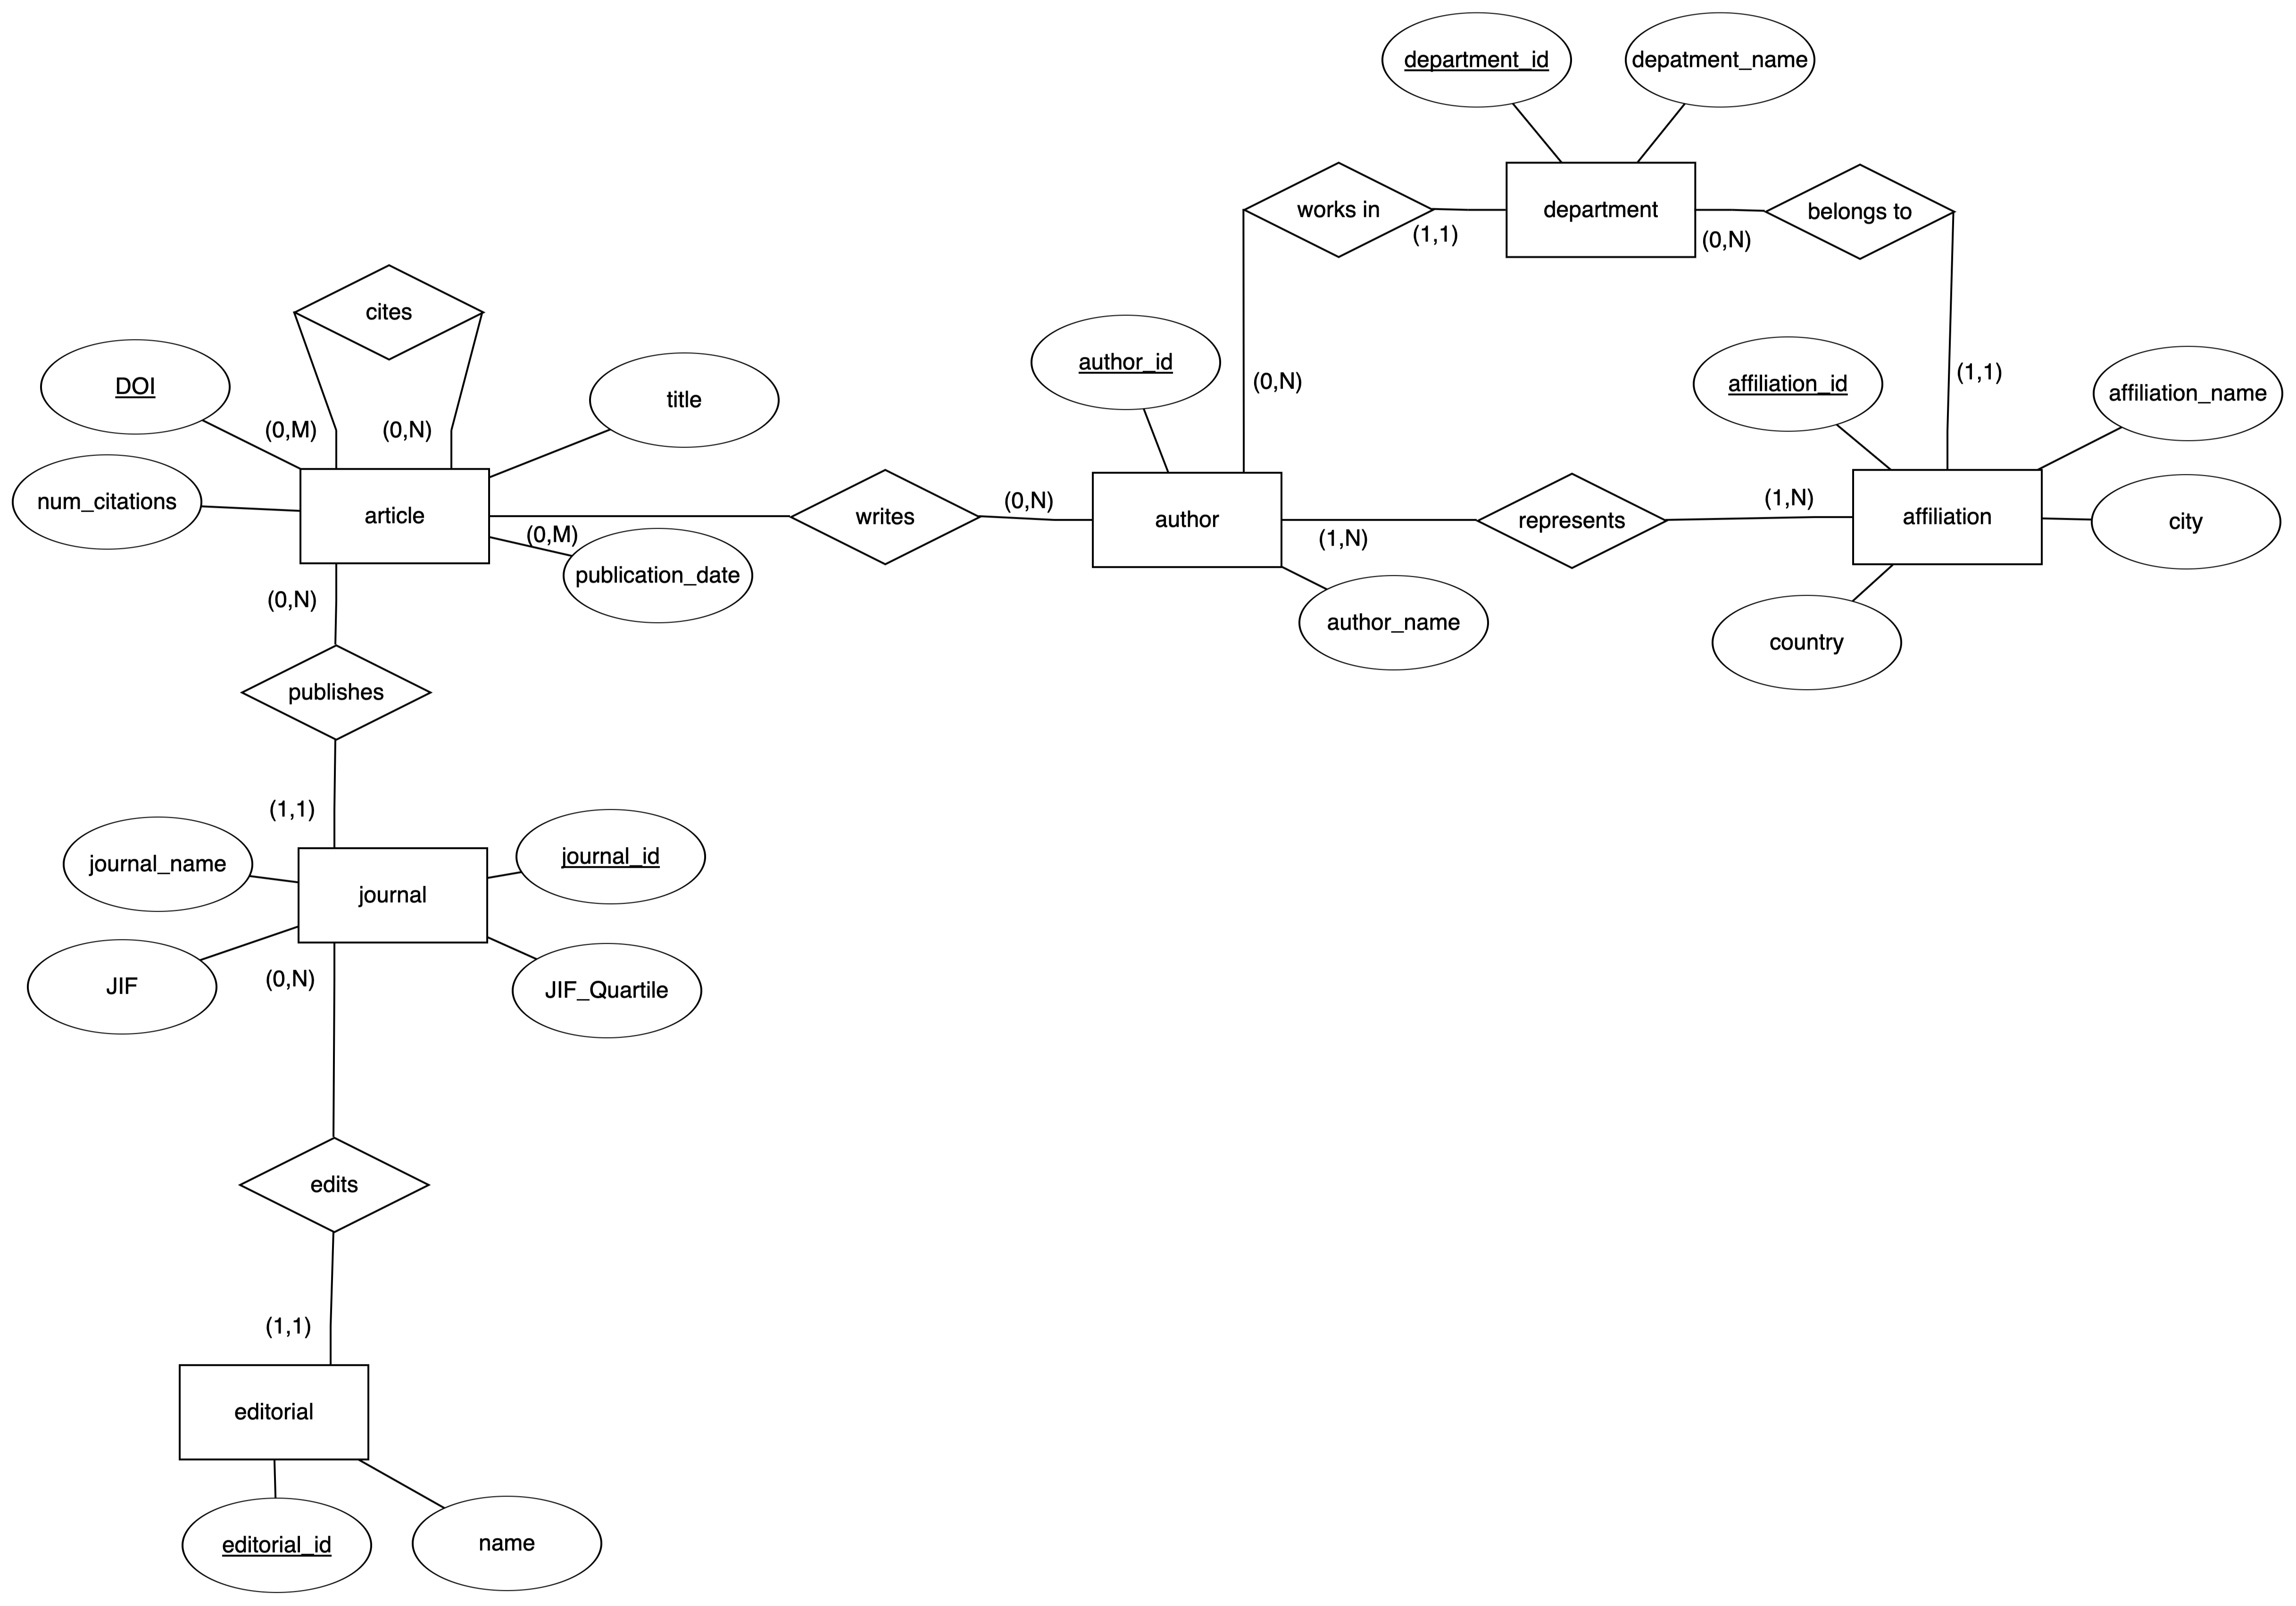
\includegraphics[width=1\textwidth]{figs/bbdd_curso-2023-2024_extraordinaria/erd_sol_ex1.png}

Cardinalidades mínimas:
\begin{itemize}
    \item Un autor debe pertenecer al menos a una afiliación, puesto que para poder publicar es necesario estar vinculado con algún organismo.
    \item Un autor debe trabajar en al menos un departamento, ya que no está permitido que autores publiquen sin pertenecer a alguno.
    \item Un departamento debe estar afiliado en al menos una afiliación, ya que un departamento debe pertenecer a una organización, no puede ser independiente.
    \item Un artículo debe publicarse en al menos un \textit{journal}, puesto que para realizar el acto de publicar es necesario que se publiquen en algún lugar.
\end{itemize}

\end{solution}

\newpage
\question[2\half] \textbf{Álgebra relacional y SQL.}

Una editorial académica dispone de una base de datos relacional compuesta por las siguientes \textbf{tablas} en las que recoge información sobre sus revistas (\texttt{JOURNAL}) y artículos publicados en las mismas. 
  
\textit{NOTA: El subrayado continuo indica PK (clave primaria), mientras que la cursiva indica FK (clave foránea) con referencia a la PK con la que comparte nombre.}

\texttt{KEYWORDS(\underline{keyword\_id}, keyword\_name)}
\vspace{1em}

\texttt{ARTICLE\_KEYWORDS(\underline{\textit{DOI}}, \underline{\textit{keyword\_id}})}
\vspace{1em}

\texttt{ARTICLE(\underline{DOI}, title, date\_published, \textit{journal\_id})}
\vspace{1em}

\texttt{JOURNAL(\underline{journal\_id}, journal\_name, IF)}
\vspace{1em}

\texttt{JOURNAL\_TOPIC(\underline{\textit{journal\_id}}, \underline{\textit{topic\_id}})}
\vspace{1em}

\texttt{TOPIC(\underline{topic\_id}, topic\_name)}
\vspace{1em}

\texttt{AUTHOR(\underline{author\_id}, name)}
\vspace{1em}

\texttt{AUTHOR\_ARTICLE(\underline{\textit{DOI}},\underline{\textit{author\_id}})}
\vspace{1em}

\texttt{CITATIONS(\underline{\textit{DOI\_citing}},\underline{\textit{DOI\_cited}})}
\vspace{1em}

\begin{parts}

\part[\half] Álgebra relacional
\begin{subparts}

\subpart[\half] Obtener el nombre de los \textit{journals} que solamente han publicado artículos a partir del año 2023 (del 2023 incluido en adelante). Considere para ello que todos los \textit{journals} han publicado al menos un artículo.

\begin{solution}[13em]
\begin{equation*}
\begin{aligned}
\Pi_{journal\_name} ( 
[ \Pi_{journal\_id} (Journal) - \\
\Pi_{journal\_id} \left(\sigma_{date\_published < 2023} (Article) \right) ] \bowtie Journal )
\end{aligned}
\end{equation*}
\end{solution}

\end{subparts}
    
\part[2] SQL
\begin{subparts}

\subpart[\half] Obtener el DOI, el título del artículo y número de \textit{keywords} de los artículos que tengan el mayor número de \textit{keywords} de la base de datos.

\begin{solution}[16em]
\begin{lstlisting}[language=SQL]
SELECT a.DOI, a.title, COUNT(*)
FROM article a 
    INNER JOIN article_keywords ak ON a.DOI = ak.DOI
GROUP BY a.DOI, a.title
HAVING COUNT(*) >= ALL(SELECT COUNT(*) 
                       FROM article_keywords 
                       GROUP BY DOI);
\end{lstlisting}
\end{solution}

\subpart[\half] Obtener el nombre de los \textit{journals} que hayan publicado en todos los \textit{topics}.

\begin{solution}[16em]
\begin{lstlisting}[language=SQL]
SELECT j.journal_name
FROM JOURNAL j
WHERE NOT EXISTS (
  SELECT t.topic_id
  FROM TOPIC t
  WHERE NOT EXISTS (
      SELECT *
      FROM JOURNAL_TOPIC jt
      WHERE jt.journal_id = j.journal_id
        AND jt.topic_id = t.topic_id
  )
);
\end{lstlisting}
\end{solution}

\subpart[\half] Obtener el título de los artículos que no fueron publicados en \textit{journals} con el \textit{topic} ``bases de datos'' durante el año 2023 (desde el 01/01/2023 hasta el 31/12/2023).

\begin{solution}[16em]
\begin{lstlisting}[language=SQL]
SELECT a.title 
FROM article a
WHERE a.date_published >= '2023-01-01' 
AND a.date_published <= '2023-12-31'
AND a.journal_id NOT IN (
    SELECT jt.journal_id
    FROM journal_topic jt
        INNER JOIN topic t ON jt.topic_id = t.topic_id
    WHERE t.topic_name = 'bases de datos');
\end{lstlisting}
\end{solution}

\subpart[\half] Obtener el título de los artículos que no contienen las keywords ``machine learning'' ni ``deep learning''.

\begin{solution}[16em]
\begin{lstlisting}[language=SQL]
SELECT a.title 
FROM article a
INNER JOIN article_keywords ak ON a.DOI = ak.DOI
INNER JOIN keywords k ON ak.keyword_id = k.keyword_id
WHERE a.DOI NOT IN (
  SELECT ak.DOI
  FROM article_keywords ak
    INNER JOIN keywords k ON ak.keywords_id = k.keywords_id
  WHERE k.keyword_name = 'machine learning')
AND a.DOI NOT IN (    
  SELECT ak.DOI
  FROM article_keywords ak
    INNER JOIN keywords k ON ak.keywords_id = k.keywords_id
  WHERE k.keyword_name = 'deep learning');
\end{lstlisting}
\end{solution}

\end{subparts}
\end{parts}

\newpage
\question[2\half] \textbf{Procedimientos, triggers y funciones.}

La editorial descrita en el ejercicio 2 quiere mantener unos estándares de calidad científica y para ello, entre otras cosas, ha definido una política de concienciación sobre las autocitas excesivas (autores en cuyos artículos referencian a otros artículos del mismo autor). Esta política consiste en detectar si un autor tiene un 20\% o más de autocitas sobre el total de citas del artículo que se ha publicado, y en ese caso, avisar a dichos autores. La primera acción realizada ha sido añadir una nueva columna llamada \textit{self\_citations} a la tabla \texttt{AUTHOR\_ARTICLE} para registrarlo.


\begin{parts}
\part[\half] Función: programe una función \texttt{get\_self\_citations} en SQL que reciba el identificador de un artículo (\texttt{DOI}) y un identificador de un autor (\texttt{author\_id}) y devuelva un número entero con el número de veces que el autor se ha citado a sí mismo dentro de ese artículo.

\begin{solution}[37em]
\begin{lstlisting}[language=SQL]
DELIMITER &&
CREATE FUNCTION get_self_citations(id_art INT, id_au INT)
RETURNS INT
DETERMINISTIC
BEGIN
    DECLARE autocitas INT DEFAULT 0;
    SELECT COUNT(*) INTO autocitas
    FROM AUTHOR_ARTICLE 
        JOIN CITATIONS 
            ON AUTHOR_ARTICLE.DOI = CITATIONS.DOI_cited
    WHERE CITATIONS.DOI_citing = id_art
      AND AUTHOR_ARTICLE.author_id = id_au;
    RETURN (autocitas);
END&&
DELIMITER ;
\end{lstlisting}
\end{solution}

\part[1] Procedmiento: programe un procedimiento en SQL sin parámetros de entrada ni de salida, que utilice un cursor para recorrer las tuplas de la tabla \texttt{AUTHOR\_ARTICLE}, calcule el número de autocitas del autor en su artículo (utilizando la función anterior), y por último, rellene la nueva columna \texttt{self\_citations} de la tabla que se creó tal y como se especificó en el enunciado de este ejercicio. NOTA: el cursor solo debe recorrer aquellas tuplas SIN la información de las autocitas (valor NULL).
    
\begin{solution}[37em]
\begin{lstlisting}[language=SQL]
DELIMITER &&
CREATE PROCEDURE fill_self_citations()
BEGIN
    DECLARE done INT DEFAULT false;
    DECLARE id_art, id_au, selfcit INT;
    DECLARE cur1 CURSOR FOR SELECT * 
                            FROM AUTHOR_ARTICLE 
                            WHERE self_citations IS NULL;
    DECLARE CONTINUE HANDLER FOR NOT FOUND SET done = true;
    OPEN cur1;
    loop1: LOOP
        FETCH cur1 INTO id_art, id_au, selfcit;
        IF done THEN
            LEAVE loop1;
        END IF;
        UPDATE AUTHOR_ARTICLE
        SET self_citations = get_self_citations(id_art, id_au)
        WHERE DOI=id_art AND author_id=id_au;
	END LOOP;
    CLOSE cur1;
END &&
DELIMITER ;
\end{lstlisting}
\end{solution}

\part[1] Trigger: programe un trigger en el que cada vez que se actualice la tabla \texttt{AUTHOR\_ARTICLE} con la información de las autocitas, se calcule el porcentaje de autocitas sobre el total de citas que tiene ese artículo (\texttt{num\_citations}) y en caso de superar el porcentaje del 20\%, impida la inserción y devuelva un ERROR con un mensaje donde aparezca el \texttt{author\_id} del autor que viole esta política (puede para ello usar el método \texttt{concat()}).
    
\begin{solution}[30em]
\begin{lstlisting}[language=SQL]
DELIMITER &&
CREATE TRIGGER check_self_citations 
BEFORE UPDATE ON AUTHOR_ARTICLE
FOR EACH ROW
BEGIN
  DECLARE n_cit INT DEFAULT 0;
  DECLARE error_msg VARCHAR(250);
  
  SELECT COUNT(*) INTO n_cit
  FROM CITATIONS
  WHERE DOI_citing = NEW.DOI;
  
  IF (NEW.self_citations IS NOT NULL) THEN
    IF (NEW.self_citations/n_cit >= 0.2) THEN
      SET error_msg = concat('The author ', NEW.author_id, 
       ' has exceeded the self-citations ratio in article ', NEW.DOI);
      SIGNAL SQLSTATE '45000'
      SET MESSAGE_TEXT = error_msg;
    END IF;
  END IF;
END &&
DELIMITER ;
\end{lstlisting}
\end{solution}
\end{parts}

\newpage
\question[1] \textbf{Control de acceso.}

Cree una vista en SQL que permita conocer el número de artículos publicados por cada \texttt{journal} del modelo de base de datos del ejercicio 2. Las columnas de la vista deberán ser el nombre del journal (\texttt{journal\_name}) y el número total de artículos publicados. A continuación, cree un usuario denominado `\texttt{consultor}' y otorguele únicamente permisos de consulta sobre esa vista.
        
\begin{solution}[16em]
\begin{lstlisting}[language=SQL]
CREATE VIEW num_articles AS 
SELECT journal_name, COUNT(*)
FROM article NATURAL JOIN journal
GROUP BY journal_id, journal_name;

CREATE USER 'consultor' IDENTIFIED BY '1234';

GRANT SELECT ON num_articles TO 'consultor';
\end{lstlisting}
\end{solution}

\newpage
\question[1] \textbf{Programación contra bases de datos.}

Realiza el etiquetado de clases y sus atributos para que mediante el ORM Hibernate de Java se pueda realizar la conexión con la base de datos satisfactoriamente cumpliendo con el \textbf{modelo relacional mostrado en el ejercicio 2}. Ten en cuenta que las claves numéricas deberán generarse automáticamente y que los atributos de nombre no pueden ser nulos.

\textbf{No repliques el código}. Incluye las anotaciones en el código Java que se muestra a continuación.

\textit{NOTA: Con el fin de simplificar la solución, algunas relaciones presentes en el modelo relacional del ejercicio 2 han sido intencionadamente excluidas en el código de este ejercicio. Utiliza únicamente las clases y atributos proporcionados.}

\begin{verbatim} 


public class Journal {

  
    private Long id;

    
    private String name;


    private Float impactFactor;


    private Set<Article> articles;


    private Set<Topic> topics;
}


public class Article {

    
    private String doi;

    
    private String title;


    private Date datePublished;


    private Journal journal;
    
}


public class Topic {


    private Long id;


    private String name;


    private Set<Journal> journals;
}
\end{verbatim}
    

\begin{solutionorbox}
\begin{verbatim} 
@Entity
@Table(name = "JOURNAL")
public class Journal {
    @Id
    @GeneratedValue
    @Column(name = "journal_id")
    private Long id;

    @Column(name = "journal_name", nullable = false)
    private String name;

    @Column(name = "impactFactor")
    private Float impactFactor;

    @OneToMany(mappedBy = "journal")
    private Set<Article> articles;

    @ManyToMany
    @JoinTable(name = "JOURNAL_TOPIC", 
                joinColumns = @JoinColumn(name = "journal_id"))
    private Set<Topic> topics;
}

@Entity
@Table(name = "ARTICLE")
public class Article {
    @Id
    @Column(name = "DOI", nullable = false)
    private String doi;

    @Column(name = "title", nullable = false)
    private String title;

    @Column(name = "date_published")
    @Temporal(TemporalType.DATE)
    private Date datePublished;

    @ManyToOne
    @JoinColumn(name = "journal_id", nullable = false)
    private Journal journal;
}

@Entity
@Table(name = "TOPIC")
public class Topic {
    @Id
    @GeneratedValue
    @Column(name = "topic_id")
    private Long id;

    @Column(name = "topic_name", nullable = false)
    private String name;

    @ManyToMany(mappedBy = "topics")
    private Set<Journal> journals;
}
\end{verbatim}
\end{solutionorbox}


\end{questions}
\end{document}